% +------------------------------------------------------------------------+
% | Reference manual page: Subdivision_method_3.tex
% +------------------------------------------------------------------------+
% | 03/01/2005   Le-Jeng Andy Shiue
% | Package: Subdivision_surface_3
% | 
\RCSdef{\RCSSubdivisionRev}{$Id$}
\RCSdefDate{\RCSSubdivisionDate}{$Date$}
% +------------------------------------------------------------------------+

\ccRefPageBegin

%%RefPage: end of header, begin of main body
% +------------------------------------------------------------------------+


\begin{ccRefClass}{Subdivision_method_3}

\ccDefinition

A subdivision method recursively refines a coarse mesh and 
generates an ever closer approximation to a smooth surface.
\ccClassTemplateName\ consists of four subdivision methods
and their refinement hosts. Each refinement host is a function 
with template parameters of a polyhedron class and a 
geometry policy class. It refines the connectivity of the
control mesh and computes the geometry of the refined mesh.
The geometry computation is dedicated to the user-customizable
geometry policy. The geometry policy consists of a set of functions 
computing the new points based on a specific subdivision stencil.
A stencil defines the footprint (a submesh of the control mesh)
of the new point.

The four supported refinbement hosts are the 
Primal-Quadrilateral-Quadrisection (PQQ),
the Primal-Triangle-Quadrisection (PTQ), 
the Dual-Quadrilateral-Quadrisection (DQQ), 
and the $\sqrt{3}$ triangulation.
Each of these refinements are respectively used in 
Catmull-Clark, Loop, Doo-Sabin and $\sqrt{3}$ subdivision, which
are also supported by \ccClassTemplateName .

\ccInclude{CGAL/Subdivision_method_3.h}

% +-----------------------------------+
\ccHeading{Refinement Host}
A refinement host is a function with template parameters of 
a polyhedron class and a geometry mask class. It refines
the input polyhedron, and assigns new points by the geometry masks.
\ccc{Subdivision_method_3} supports four refinement hosts:
primal quadrilateral quadrisection (PQQ), 
primal triangle quadrisection (PTQ), dual quadrilateral 
quadrisection (DQQ) and $\sqrt{3}$ triangulation.

\begin{ccTexOnly}
  \begin{center}
    \parbox{0.6\textwidth}{%
      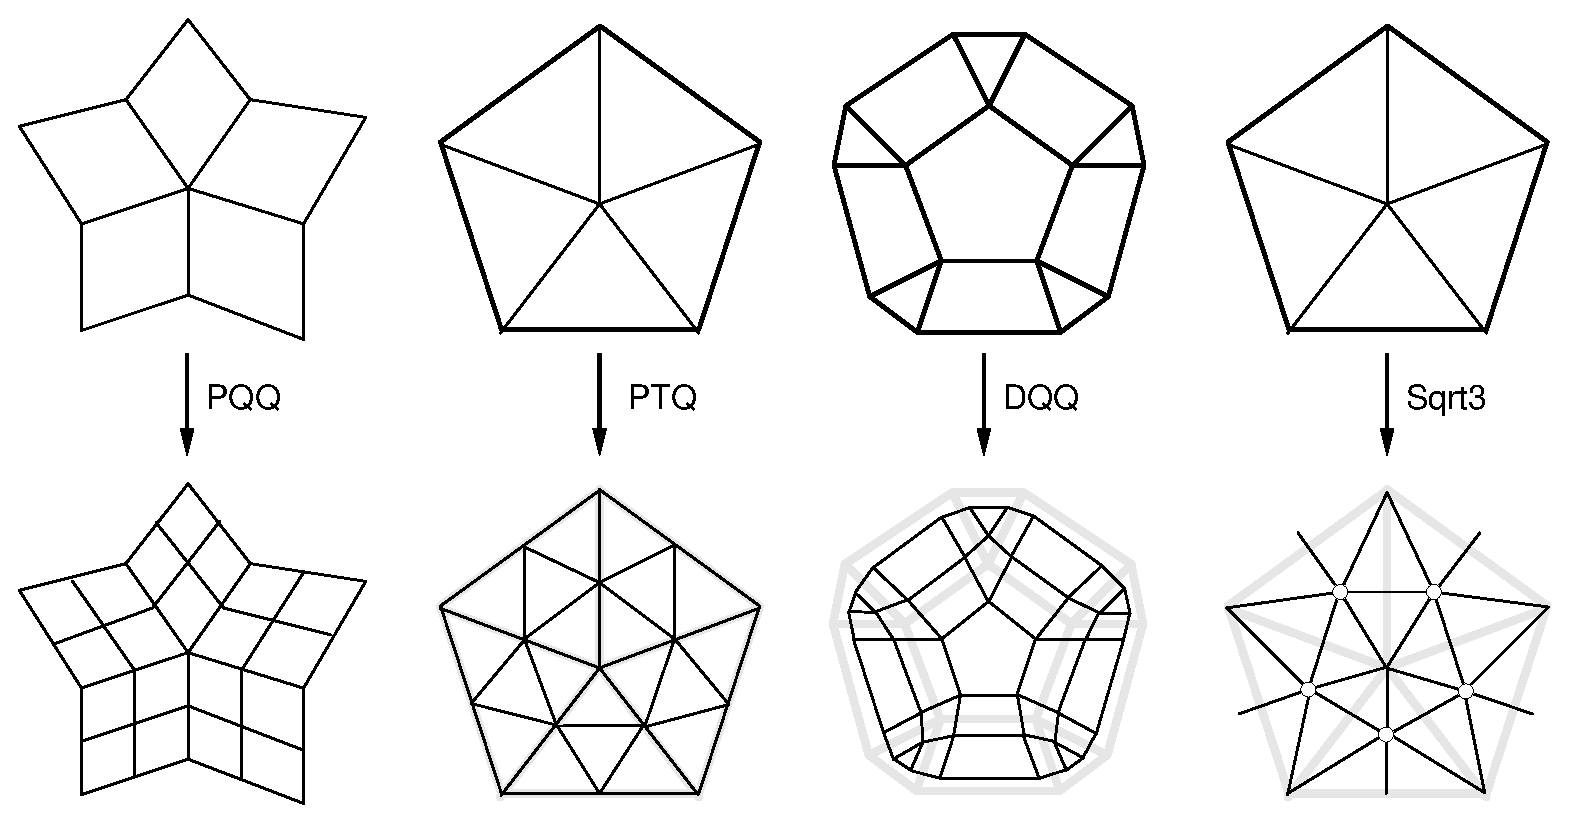
\includegraphics[width=0.6\textwidth]{Subdivision_method_3_ref/FIG/RefSchemes}%
    }\\ \vspace{0.5cm}
  \end{center}
\end{ccTexOnly}

\begin{ccHtmlOnly}
  <CENTER>
     <img src="FIG/RefSchemes.gif" alt="Refinement Hosts"><P>
  </CENTER>
\end{ccHtmlOnly}

%\ccThree{void}{S::PQQ(Poly& p, Stencil<Poly> rule, int s);}{}
%\ccThreeToTwo
\ccTwo{template <template <typename> class Stencil> void PQQ(Poly& p, Stencil<Poly> rule, int s);}{}

\ccThree{template <template <typename> class Stencil> void}{sub}{}
\ccThreeToTwo


\ccFunction{
template <class Polyhedron, template <typename> class Mask>
void PQQ(Polyhedron& p, Mask<Polyhedron> mask, int step = 1);
}{
apply the PQQ refinement on the control mesh \ccc{p} \ccc{step} times.
The geometry of the refined mesh is computed by the geometry policy \ccc{mask}
This function overwrites the control mesh \ccc{p} with the refined mesh.
}

\ccFunction{
template <class Polyhedron, template <typename> class Mask>
void PTQ(Polyhedron& p, Mask<Polyhedron> mask, int step = 1);
}{
apply the PTQ refinement on the control mesh \ccc{p} \ccc{step} times.
The geometry of the refined mesh is computed by the geometry policy \ccc{mask}
This function overwrites the control mesh \ccc{p} with the refined mesh.
}

\ccFunction{
template <class Polyhedron, template <typename> class Mask>
void DQQ(Polyhedron& p, Mask<Polyhedron> mask, int step = 1);
}{
apply the DQQ refinement on the control mesh \ccc{p} \ccc{step} times.
The geometry of the refined mesh is computed by the geometry policy \ccc{mask}
This function overwrites the control mesh \ccc{p} with the refined mesh.
}

\ccFunction{
template <class Polyhedron, template <typename> class Mask>
void Sqrt3(Polyhedron& p, Mask<Polyhedron> mask, int step = 1);
}{
apply the $\sqrt{3}$ triangulation on the control mesh \ccc{p} \ccc{step} times.
The geometry of the refined mesh is computed by the geometry policy \ccc{mask}
This function overwrites the control mesh \ccc{p} with the refined mesh.
}

% +-----------------------------------+
\ccHeading{Subdivision Method}

%\ccTwo{void CatmullClark_subdivision(Poly& p, int d);}{}
\ccThree{void}{sub}{}
\ccThreeToTwo

\ccFunction{
template <class Polyhedron>
void CatmullClark_subdivision(Polyhedron& p, int step = 1);
}{
apply Catmull-Clark subdivision \ccc{step} times on the control mesh \ccc{p}.
The control mesh \ccc{p} is overwritten with the subdivided mesh.
}

\ccFunction{
template <class Polyhedron>
void Loop_subdivision(Polyhedron& p, int step = 1); 
}{
apply Loop subdivision \ccc{step} times on the control mesh \ccc{p}.
The control mesh \ccc{p} is overwritten with the subdivided mesh.
}

\ccFunction{
template <class Polyhedron>
void DooSabin_subdivision(Polyhedron& p, int step = 1);
}{
apply Doo-Sabin subdivision \ccc{step} times on the control mesh \ccc{p}.
The control mesh \ccc{p} is overwritten with the subdivided mesh.
}

\ccFunction{
template <class Polyhedron>
void Sqrt3_subdivision(Polyhedron& p, int step = 1);
}{
apply $\sqrt{3}$ subdivision \ccc{step} times on the control mesh \ccc{p}.
The control mesh \ccc{p} is overwritten with the subdivided mesh.
}

\ccSeeAlso

\ccRefIdfierPage{CGAL::PQQ_stencil_3<Polyhedron>}\\
\ccRefIdfierPage{CGAL::DQQ_stencil_3<Polyhedron>}\\
\ccRefIdfierPage{CGAL::Linear_mask_3<Polyhedron>}\\
\ccRefIdfierPage{CGAL::CatmullClark_mask_3<Polyhedron>}\\
\ccRefIdfierPage{CGAL::Loop_mask_3<Polyhedron>}\\
\ccRefIdfierPage{CGAL::Sqrt3_mask_3<Polyhedron>}\\

\ccExample

This example program subdivides a polyhedral mesh with
Catmull-Clark subdivision.

\ccIncludeExampleCode{Subdivision_method_3/CatmullClark_subdivision.C}

\end{ccRefClass}

% +------------------------------------------------------------------------+
%%RefPage: end of main body, begin of footer
\ccRefPageEnd
% EOF
% +------------------------------------------------------------------------+
